\documentclass[twocolumn,letterpaper,aps,pra,10pt]{revtex4-1}
\usepackage[spanish]{babel}
\usepackage[utf8]{inputenc}
\usepackage[T1]{fontenc}
\usepackage{times}
\usepackage{calligra}
\usepackage{graphicx}
\usepackage{latexsym}
\usepackage{amsmath,amssymb}
\usepackage{subfigure}
\usepackage{booktabs}
\usepackage{tabulary}
\usepackage{url}
%\usepackage{mhchem}
\spanishdecimal{.}
\usepackage{ragged2e}
\bibliographystyle{unsrt}
\usepackage[usenames,dvipsnames]{pstricks}
\usepackage{epsfig}
\usepackage{pst-grad} % For gradients
\usepackage{pst-plot} % For axes
\usepackage{float}
\usepackage{colortbl}
\usepackage{hyperref}
\usepackage{latexsym}
\usepackage{xcolor}
\usepackage{fancyhdr}
\pagestyle{fancy}

\begin{document}
\renewcommand{\figurename}{{\bf Figura }}
\renewcommand{\tablename}{{\bf Tabla}}
\renewcommand{\thesection}{\arabic{section}}
\renewcommand{\thesubsection}{\arabic{subsection}}

\lhead{}
\chead{}
\rhead{}
\lfoot{\thepage | F.Ciencias, IF-UNAM} 
\cfoot{}
\rfoot{Ó. Alvarado-Morán. \textit{et al.} | Gotas de agua sobre Cu, Pd y Si}

\vspace*{-1cm}
\title{Ángulo de contacto del agua sobre láminas de cobre, \\paladio y silicio con y sin grafeno.}
\author{\textbf{Ó.A. Alvarado-Morán$^{a,*}$, D.L. Monroy-Mérida$^{a,b}$, L.N. Serkovic-Loli$^{b}$}}
\affiliation{$^{a}$Facultad de Ciencias, Universidad Nacional Autónoma de México, Ciudad Universitaria, Coyoacán 04510, México.\\
$^{b}$Instituto de Física, Universidad Nacional Autónoma de México, Ciudad Universitaria, Coyoacán 04510, México.\\
$^{*}$e-mail: oscaralvarado@ciencias.unam.mx}

\begin{abstract}
En este trabajo presentamos el comportamiento de gotas de agua desionizada sobre placas de cobre, paladio y silicio con y sin grafeno para así determinar si dicho material tiene propiedades hidrofóbicas o hidrofílicas midiendo el ángulo de contacto que hace la gota de agua sobre cada sustrato. Se presenta un método para sintetizar el grafeno sobre las placas de cobre y paladio mediante el método de CVD. Los resultados obtenidos apuntan a que el grafeno dota de más propiedades hidrofóbicas a los sustratos de paladio y silicio con un aumento de ángulo de contacto de $5.318 \pm 0.0005^{o}$ y $15.045\pm 0.0005^{o}$, respectivamente. Para el cobre los resultados no son tan certeros ya que en cada ocasión de medición se obtuvieron resultados que apuntaban a propiedades tanto hidrofóbicas como hidrofílicas.
\\
\\
\textit{Palabras clave}: Ángulo de Contacto; Grafeno; CVD; Paladio.
\end{abstract}

\maketitle
%%%%%%%%%%%%%%%%%%%%%%%%%%%%%%%%%%%%%%%%%%%%%%%%%%%%%%%%%%%%%%%%%%%%%%%%%%%%%%%%%%%%%%%%%%%%%%%%%%
\section{Introducción}

Grafeno es el nombre que se le dió a una monocapa plana compuesta por átomos de carbono (puede darse en varias capas, a lo que se le llama "multicapa") empacados en un teselado hexagonal (Figura 1). Dicho material tiene propiedades muy interesantes, como ser el material más fuerte conocido hasta ahora, el más delgado (espesor de un átomo), puede aguantar densidades de corriente 6 veces más altas que las del cobre, muestra una conductividad térmica asombrosa \cite{grafeno}. Además, el transporte de electrones en el grafeno está descrito por la ecuación de Dirac. Su anchura permite aplicaciones a nanoescala. Varios materiales (como el grafito, nanotubos, etc.) son derivados del grafeno, por lo que su estudio teórico lleva ya varios años de avance\cite{grafeno2}. Por esto y más, el estudio del grafeno es importante en casi cualquier área de la ciencia y/o industria.

\begin{figure}[h]
\centering
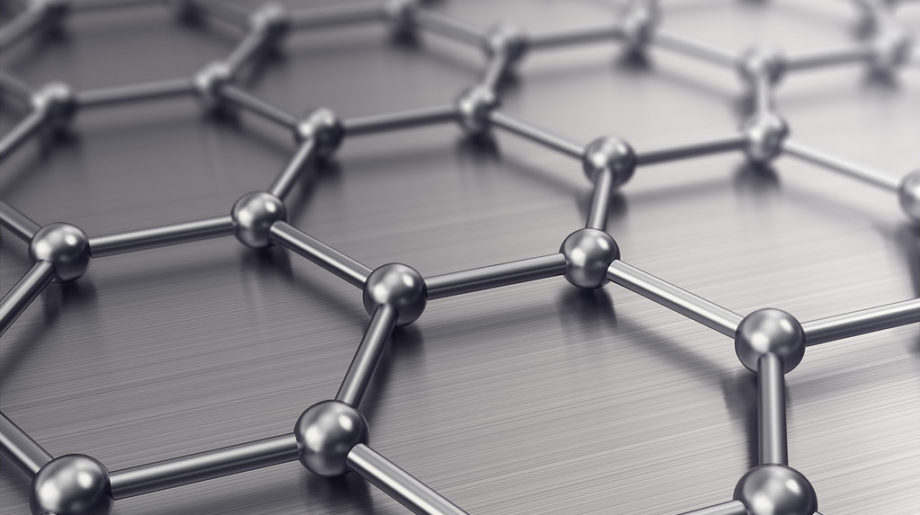
\includegraphics[scale=0.7]{grafeno-920x515.jpg}
\caption{Representación artísitica del grafeno.}
\end{figure}

El grafeno ha sido reconocido como un material hidrofóbico. Sin embargo resultados cuantitativos de sus propiedades humectantes son variados. Por lo que la caracterización de estas propiedades es un tema de interés para la investigación\cite{WCA1}. 

El ángulo de contacto es aquel ángulo que forma la superficie de un líquido, como el agua, al entrar en contacto con una superficie sólida. El valor de dicho ángulo depende de las fuerzas adhesivas entre el líquido y el sólido y las fuerzas cohesivas del líquido; cuando estas últimas son muy pequeñas respecto a las primeras, el ángulo de contacto es menor a 90 grados, lo que resulta en que el líquido moja a la superficie (Figura 2).

\begin{figure}[h]
\centering
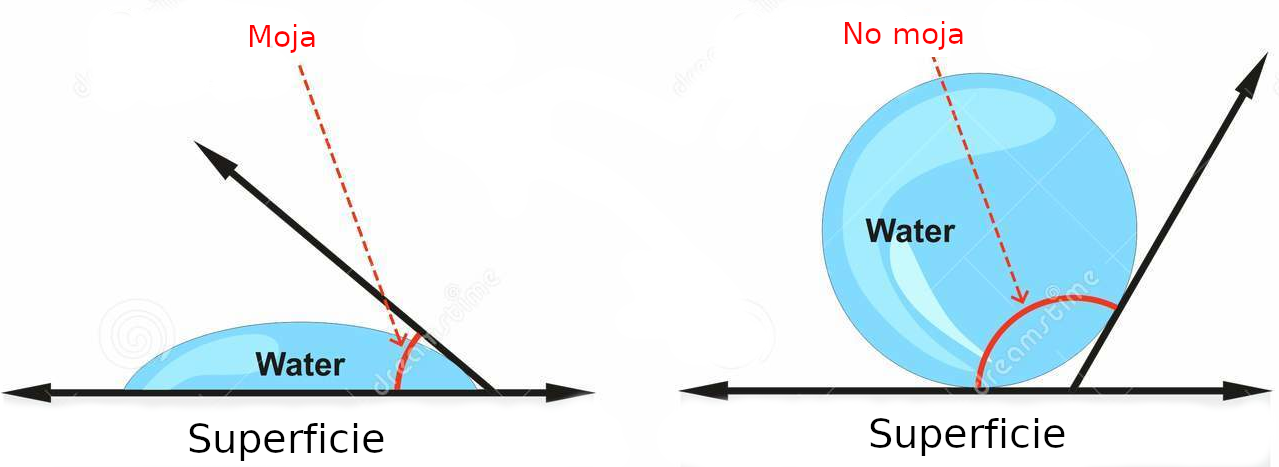
\includegraphics[scale=0.7]{AnguloMojado.png}
\caption{Se muestra el diagrama de cuando un líquido moja o no moja una superficie.}
\end{figure}


Para el grafeno se demostró que el ángulo de contacto no tiene dependencia en el grosor de las capas de dicho material depositadas sobre SiC\cite{WCA2}. Este resultado fue generalizado pero se encontró que el ángulo de contacto del agua sobre una capa de grafeno cambiaba dependiendo de el tipo de sustrato en que era depositado éste\cite{WCA3}\cite{WCA4}.
La influencia del sustrato fue eliminada al apilar varias ojuelas/capas de grafeno una encima de otra, con lo que se logró medir un ángulo de contacto de hasta 127$^{o}$. Sin embargo, dichas mediciones se hicieron con capas de grafeno unas sobre otras, y con una monocapa se encontró que el ángulo de contacto del agua sobre grafeno estaba entre los 90 y 95 grados, como pasa con el grafito \cite{WCA5}.

Para una lámina de cobre se tienen resultados experimentales de ángulo de contacto de entre $60^{o}$ y $90^{o}$ \cite{WCA6} \cite{WCA7}. Para el paladio se tienen resultados de entre $80^{o}$ y $90^{o}$\cite{WCA8}, así como para el silicio se tiene reportado un ángulo de contacto de entre $70^{o}$ y $80^{o}$\cite{WCA8}.

Se tiene la ecuación de Young-Dupré
\begin{equation}\label{Young}
W_{a}^{0} = \gamma_{LV}(1 + cos\theta ) 
\end{equation}

donde $\gamma_{LV}$ es la tensión entre las fases líquido (agua) y vapor (aire) y $\theta$ es el ángulo de contacto de equilibrio medido en el líquido. Esta ecuación describe el trabajo de adhesión del líquido al sólido, es decir, se mide qué tanto se adhiere el agua a dicho sólido\cite{YoungD}.

\textbf{Método CVD (Chemical Vapor Deposition) para producir grafeno.}\\
Antes se producía grafeno a pequeñas escalas (1000$\mu m^{2}$), debido a que sólo se podía obtener mediante exfoliación de grafito, técnica que no es fácil de llevar a gran escala. Como la industria electrónica requería grafeno de mayor área para ser manipulado se diseñaron nuevas técnicas de producción. Una de éstas es las que se conoce como CVD  (\textit{Chemical Vapor Deposition} por sus siglas en inglés). Este método involucra el flujo de un gas o gases precursores  (como metano) en una cámara que contenga uno o más objetos calientes para ser recubiertos (como láminas de cobre). Las reacciones químicas ocurren sobre las superficies calientes, teniendo como resultado que se depositen capas finas del material requerido (carbono proveniente del metano) sobre el material calentado\cite{CVD}. 
\\
\begin{figure}[h]
\centering
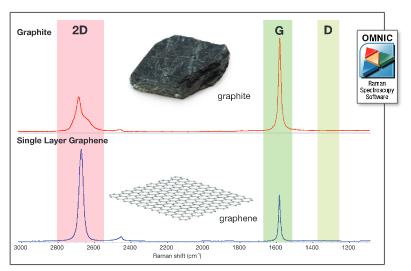
\includegraphics[scale=0.5]{Raman.png}
\caption{Espectros Raman del grafito y del grafeno (monocapa).}
\end{figure}

\textbf{Espectroscopía Raman}\\
La espectroscopía Raman es una técnica vibracional extremadamente sensible a la estructura geométrica y la unión entre moléculas. Con esta técnica, incluso diferencias pequeñas en la estructura geométrica conducen a diferencias significantes en el espectro Raman observado de una molécula. Esta sensibilidad a cambios en la estructura geométrica es bastante útil para el estudio de distintos alótropos del carbono (Figura 3), como el grafeno \cite{Raman1}.

Cuando la luz es dispersada por una molécula, la mayoría de los fotones son elásticamente se dispersados. Los fotones dispersados tienen la misma energía (frecuencia) y por lo tanto la misma longitud de onda que los fotones incidentes, sin embargo, una pequeña fracción de luz (aproximadamente $1$ en $10^{7}$ fotones) es dispersada a frecuencias ópticas distintas y usualmente menores a la frecuencia de los fotones incidentes. El proceso que lleva a esta dispersión inelástica se denomina efecto Raman.

La diferencia en energía entre el fotón incidente y el fotón dispersado Raman es igual a la energía de vibración de la molécula dispersada. Una gráfica de intensidad de luz dispersada contra diferencia de energía es un espectro Raman\cite{Raman2}.
\\
\\
{\large \textbf{Objetivos}}:
\begin{itemize}
    \item Conocer cómo varía el ángulo de contacto de gotas de agua desionizada sobre láminas de cobre, silicio y paladio con y sin grafeno.
    \item Comparar la humectabilidad de los recubrimientos de grafeno sobre los diferentes sustratos calculando el trabajo de adhesión.
    \item Determinar el grafeno como un material hidrofílico o hidrofóbico.
   
\end{itemize}
%%%%%%%%%%%%%%%%%%%%%%%%%%%%%%%%%%%%%%%%%%%%%%%%%%%%%%%%%%%%%%%%%%%%%%%%%%%%%%
\section{Procedimiento experimental}
Para ver las propiedades humectantes del grafeno sobre paladio, cobre y silicio primero se sintetizó el grafeno sobre láminas de cobre y paladio con el método de CVD, la lámina de silicio utilizada fue provista por el laboratorio donde se trabajó. Para sintetizar con el método de CVD primero se limpiaron las láminas sumergiéndolas en acetona y colocándolas en una máquina de ultrasonido durante cinco minutos, posteriormente se hizo lo mismo con isopropanol. Al terminar este proceso se secaron con nitrógeno a bajo flujo.

\begin{figure}[h]
\centering
\includegraphics[scale=0.02]{Acetona_Isopropanol.jpg}
\caption{Sustancias utilizadas para limpiar las láminas de cobre y de paladio.}
\end{figure}

Habiendo limpiado las muestras se introdujeron en el centro de un horno de tubo de vacío modelo OTF-1200 con tubo de cuarzo de 10.16cm de diámetro (véase Figura 5). 

\begin{figure}[h]
\centering
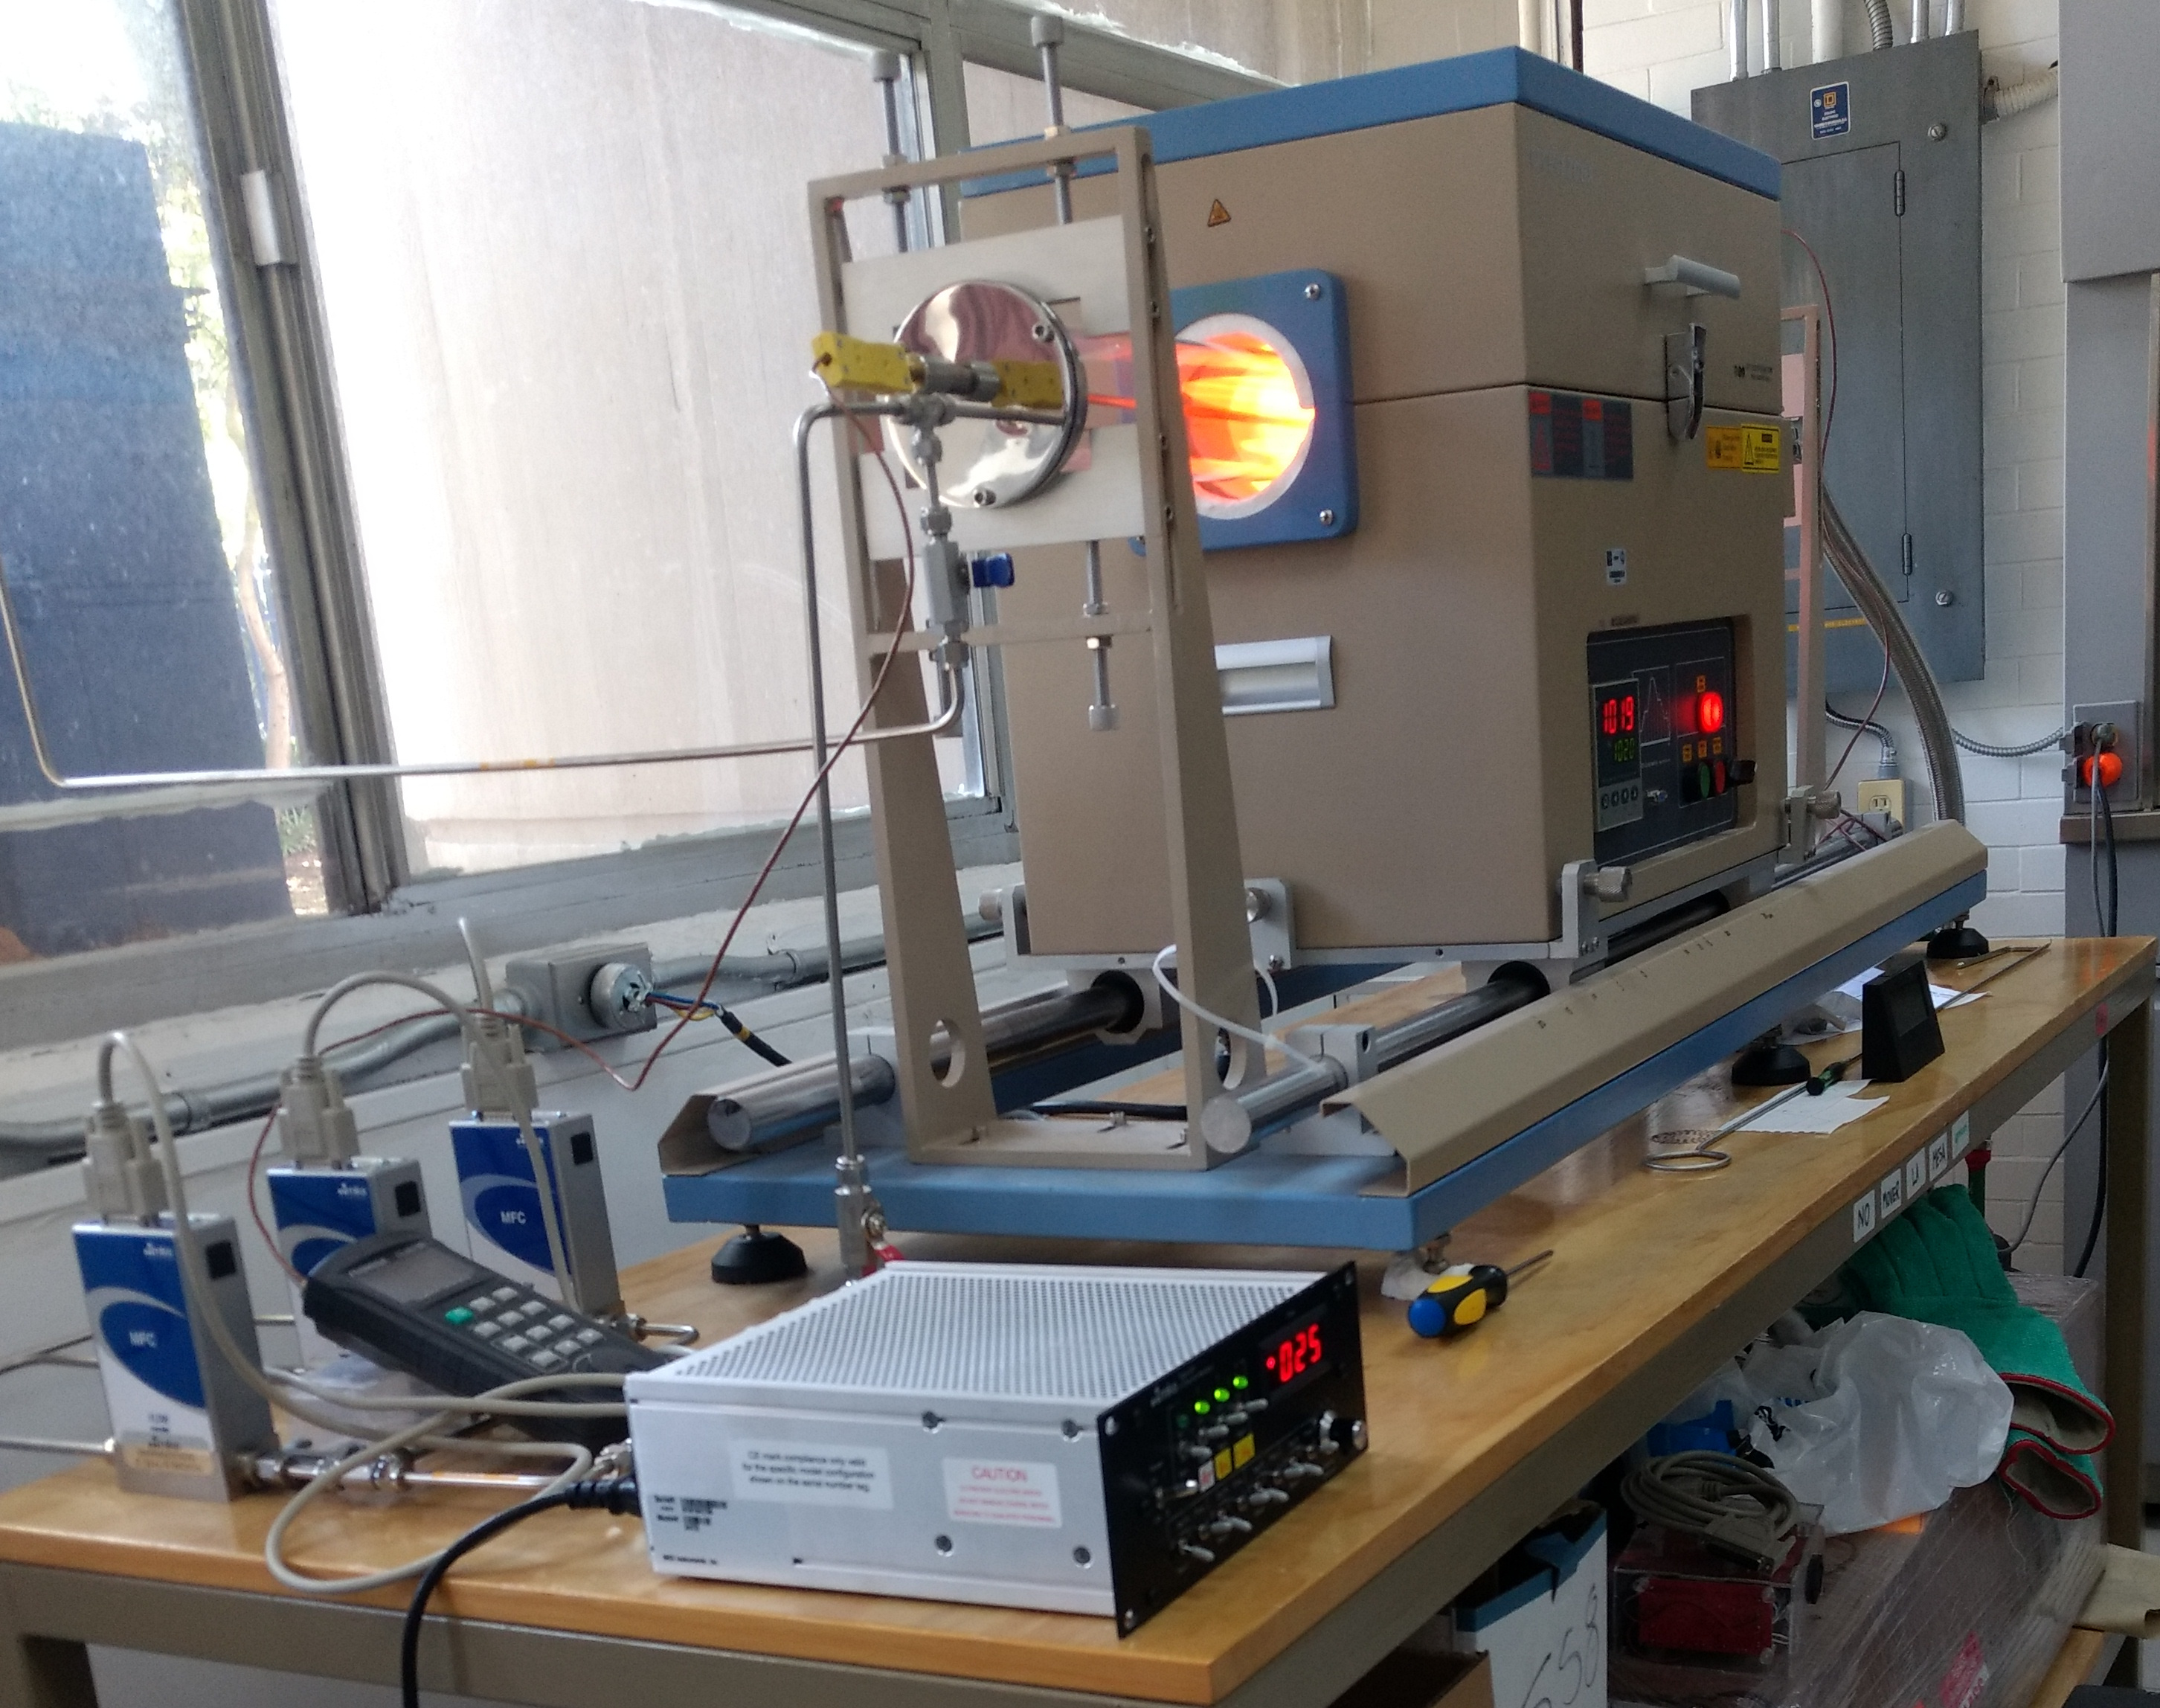
\includegraphics[scale=0.05]{Horno.jpg}
\caption{Horno utilizado durante el experimento y reguladores de flujo de masa mostrados en la parte inferior izqueirda de la imagen.}
\end{figure}

Primero se introdujeron cuatro láminas de cobre de aproximadamente $1 cm^{2}$ de área cada una; cada material lleva un proceso específico de crecimiento de grafeno en dicho horno, por lo que para las láminas de cobre se utilizaron los tiempos y las temperaturas mostradas en la Figura 6. Con un vacío en el horno de $\sim$2 Torr, un flujo continuo de hidrógeno de 70 sccm, un flujo continuo de argón de 200 sccm y un flujo de metano de 25 sccm sólo durante veinte minutos al final del procedimiento. Todas estas cantidades se regularon con varios reguladores de flujo de masa (véase Figura 5).

\begin{figure}[h]
\centering
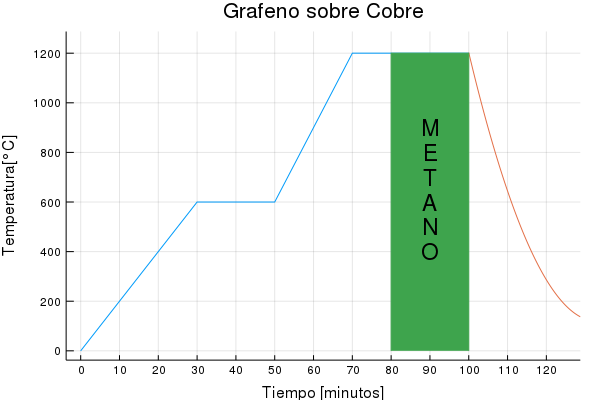
\includegraphics[scale=0.3]{Grafeno_Cobre.png}
\caption{Se muestra gráfico de Temperatura (en grados Celsius) contra tiempo (en minutos). La franja verde representa el tiempo en que se introdujo metano al horno de vacío, durante todo el tiempo hubo flujo de hidrógeno y de argón. La línea roja representa que se apagó el horno, se dejó enfríar a temperatura ambiente y que se detuvo el flujo del metano y del hidrógeno dentro del horno.}
\end{figure}

Habiendo finalizado el procedimiento con el cobre se dio paso a hacer el mismo procedimiento con el paladio pero basándose en el protocolo implementado por Gutierrez-Valdés A. et al. (2019)\cite{PaladioCVD}. Por lo que ahora los tiempos y las temperaturas utilizadas se muestran en la Figura 7. Para este caso sólo se introdujeron 2 láminas cuadradas de paladio de aproximadamente 5mm de lado. Con un vacío en el horno de $\sim$2 Torr, un flujo continuo de hidrógeno de 60 sccm, un flujo continuo de argón de 30 sccm y un flujo de metano de 50 sccm sólo durante diez minutos al final del procedimiento.

\begin{figure}[h]
\centering
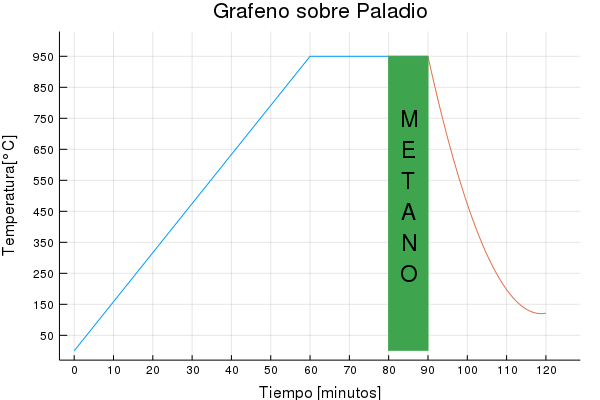
\includegraphics[scale=0.3]{Grafeno_Paladio.png}
\caption{Se muestra gráfico de Temperatura (en grados Celsius) contra tiempo (en minutos). La franja verde representa el tiempo en que se introdujo metano al horno de vacío, durante todo el tiempo hubo flujo de hidrógeno y de argón. La línea roja representa que se apagó el horno, se dejó enfríar a temperatura ambiente y que se detuvo el flujo del metano dentro del horno.}
\end{figure}

Habiendo terminado el procedimiento para los dos sustratos, se utilizo el método de espectroscopía Raman para comprobar si los protocolos implementados habían sido satisfactorios y si había grafeno sobre las láminas. Para el caso del silicio se tenía una muestra que ya se había analizado con este método y efectivamente tenía grafeno.

\begin{figure}[h]
\centering
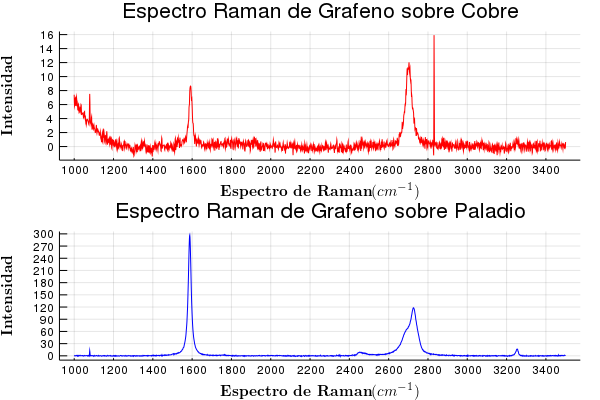
\includegraphics[scale=0.4]{Espectro_Raman.png}
\caption{a) Se muestra gráfica de el espectro Raman para grafeno sobre cobre.}
\end{figure}


Los resultados obtenidos mediante el proceso de espectroscopía Raman se muestran en la Figura 8, observando que se tiene grafeno para ambas láminas, con monocapa para el cobre y con islas de multicapas para el paladio. Imágenes con microscopio  de cada lámina cuando se tiene grafeno y cuando no se tiene se muestran en la Figuras 9.

\begin{figure}[h]
\centering
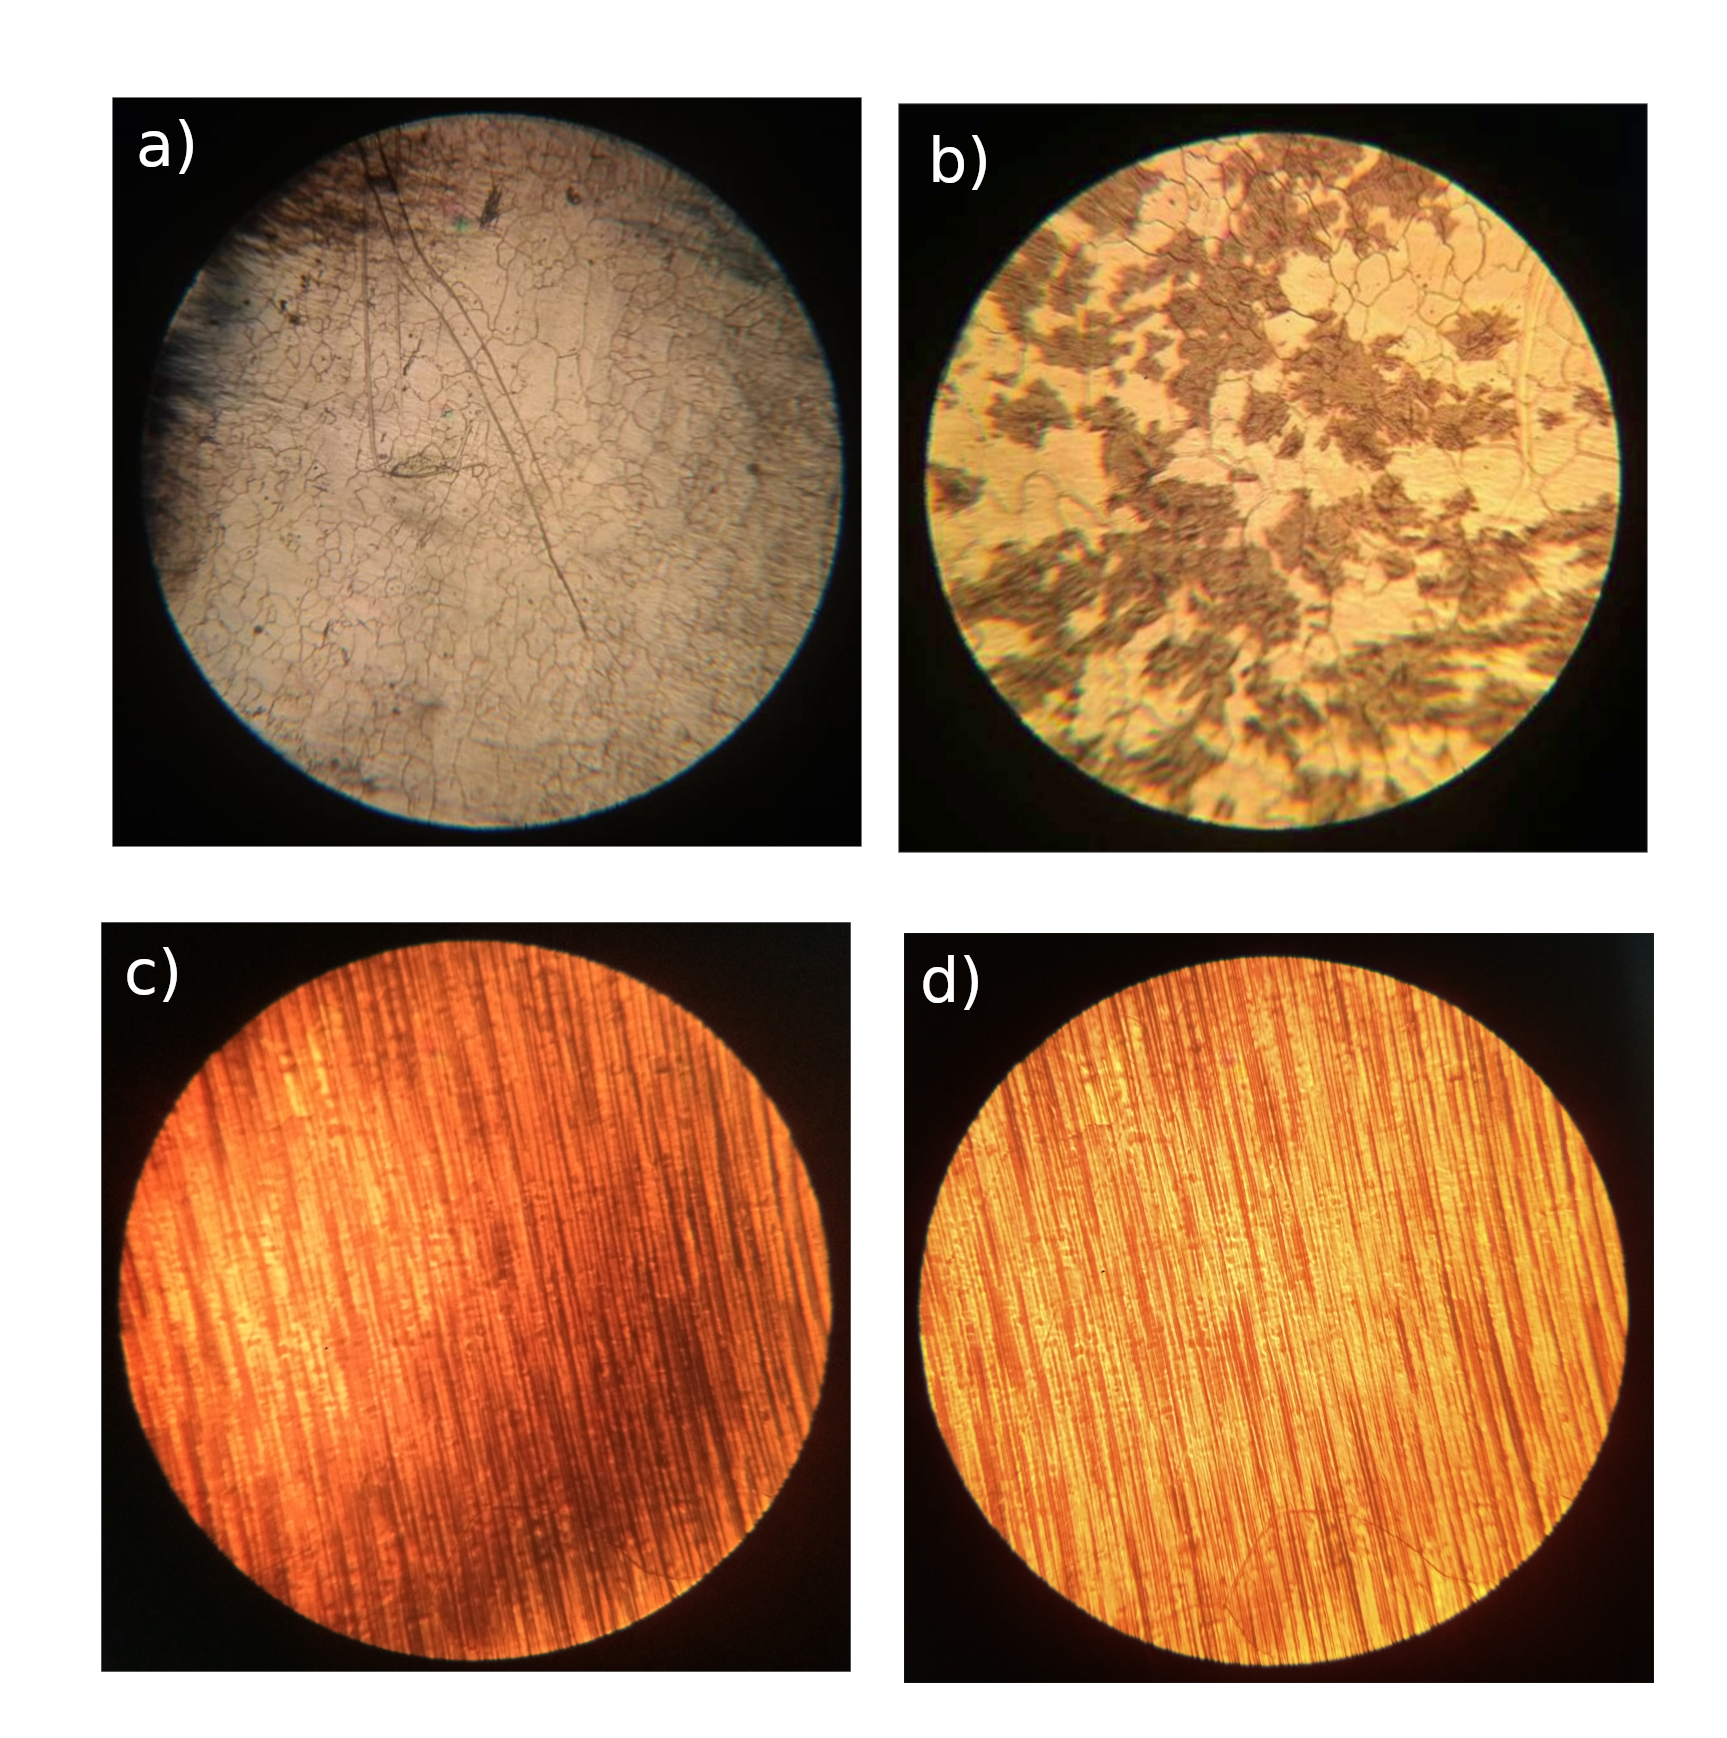
\includegraphics[scale=0.3]{Laminas_sin_con_grafeno.png}
\caption{a) Se muestra una toma con microscopio de una lámina de paladio sin grafeno sobre ésta. b) Se muestra una toma con microscopio de una lámina de paladio con grafeno sobre ésta. c) Se muestra una toma con microscopio de una lámina de cobre sin grafeno sobre ésta. d) Se muestra una toma con microscopio de una lámina de cobre con grafeno sobre ésta.}
\end{figure}

Para las láminas de silicio proporcionadas se tienen tomas con microscopio con y sin grafeno mostradas en la Figura 10

\begin{figure}[h]
\centering
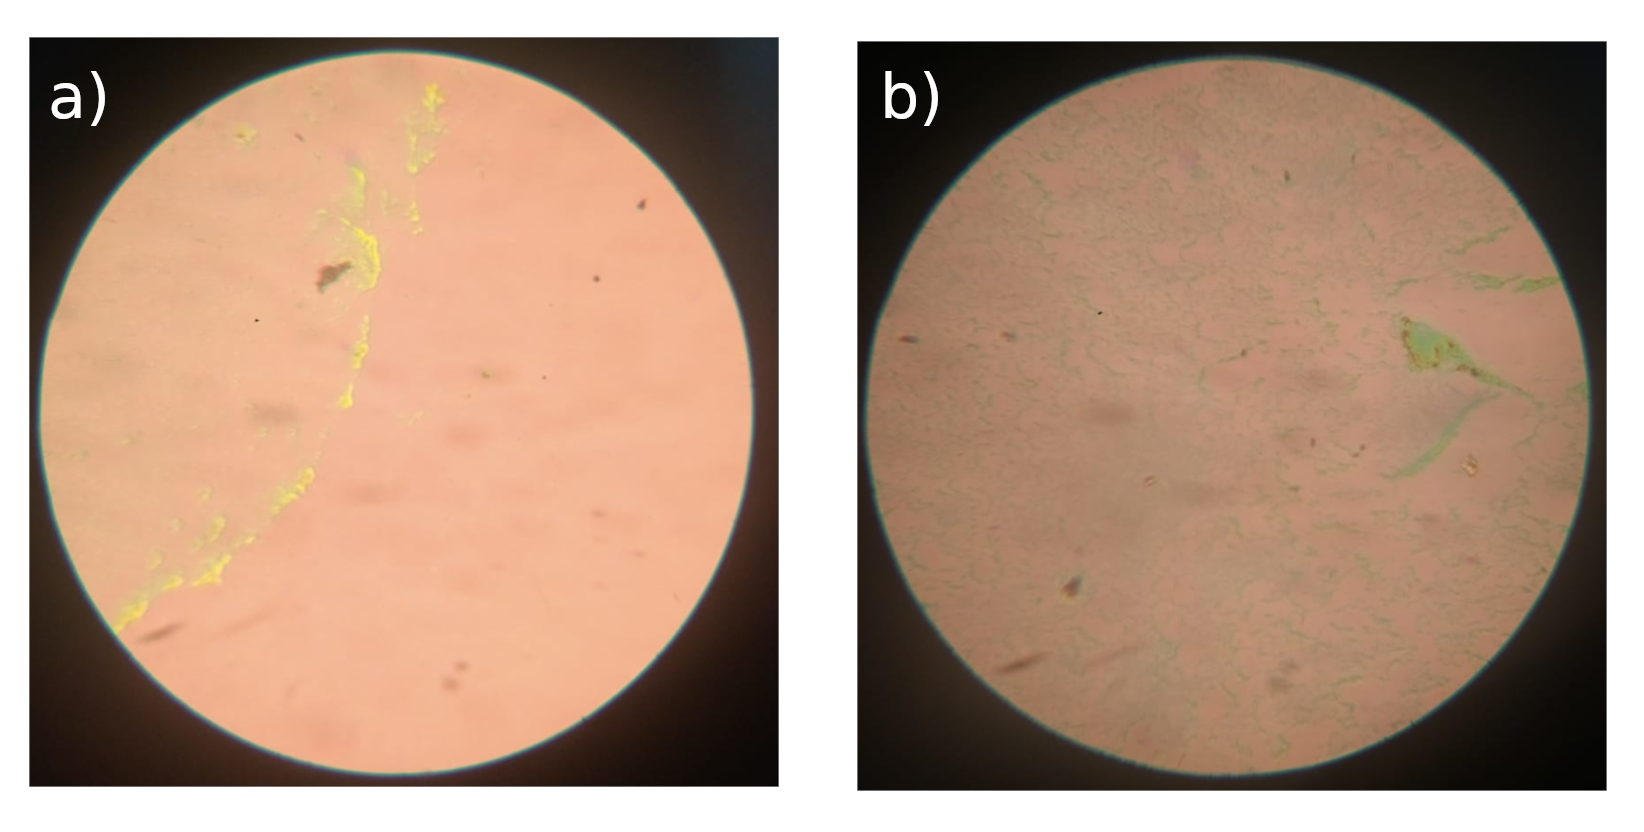
\includegraphics[scale=0.4]{Silicio_sin_con_grafeno.png}
\caption{a) Se muestra una toma con microscopio de una lámina de silicio sin grafeno sobre ésta. b) Se muestra una toma con microscopio de una lámina de silicio con grafeno sobre ésta.}
\end{figure}

Teniendo las láminas ya listas se procedió a medir sus propiedades humectantes, con lo que se desarrolló el sistema mostrado en la Figura 11. 

\begin{figure}[hbtp]
\centering
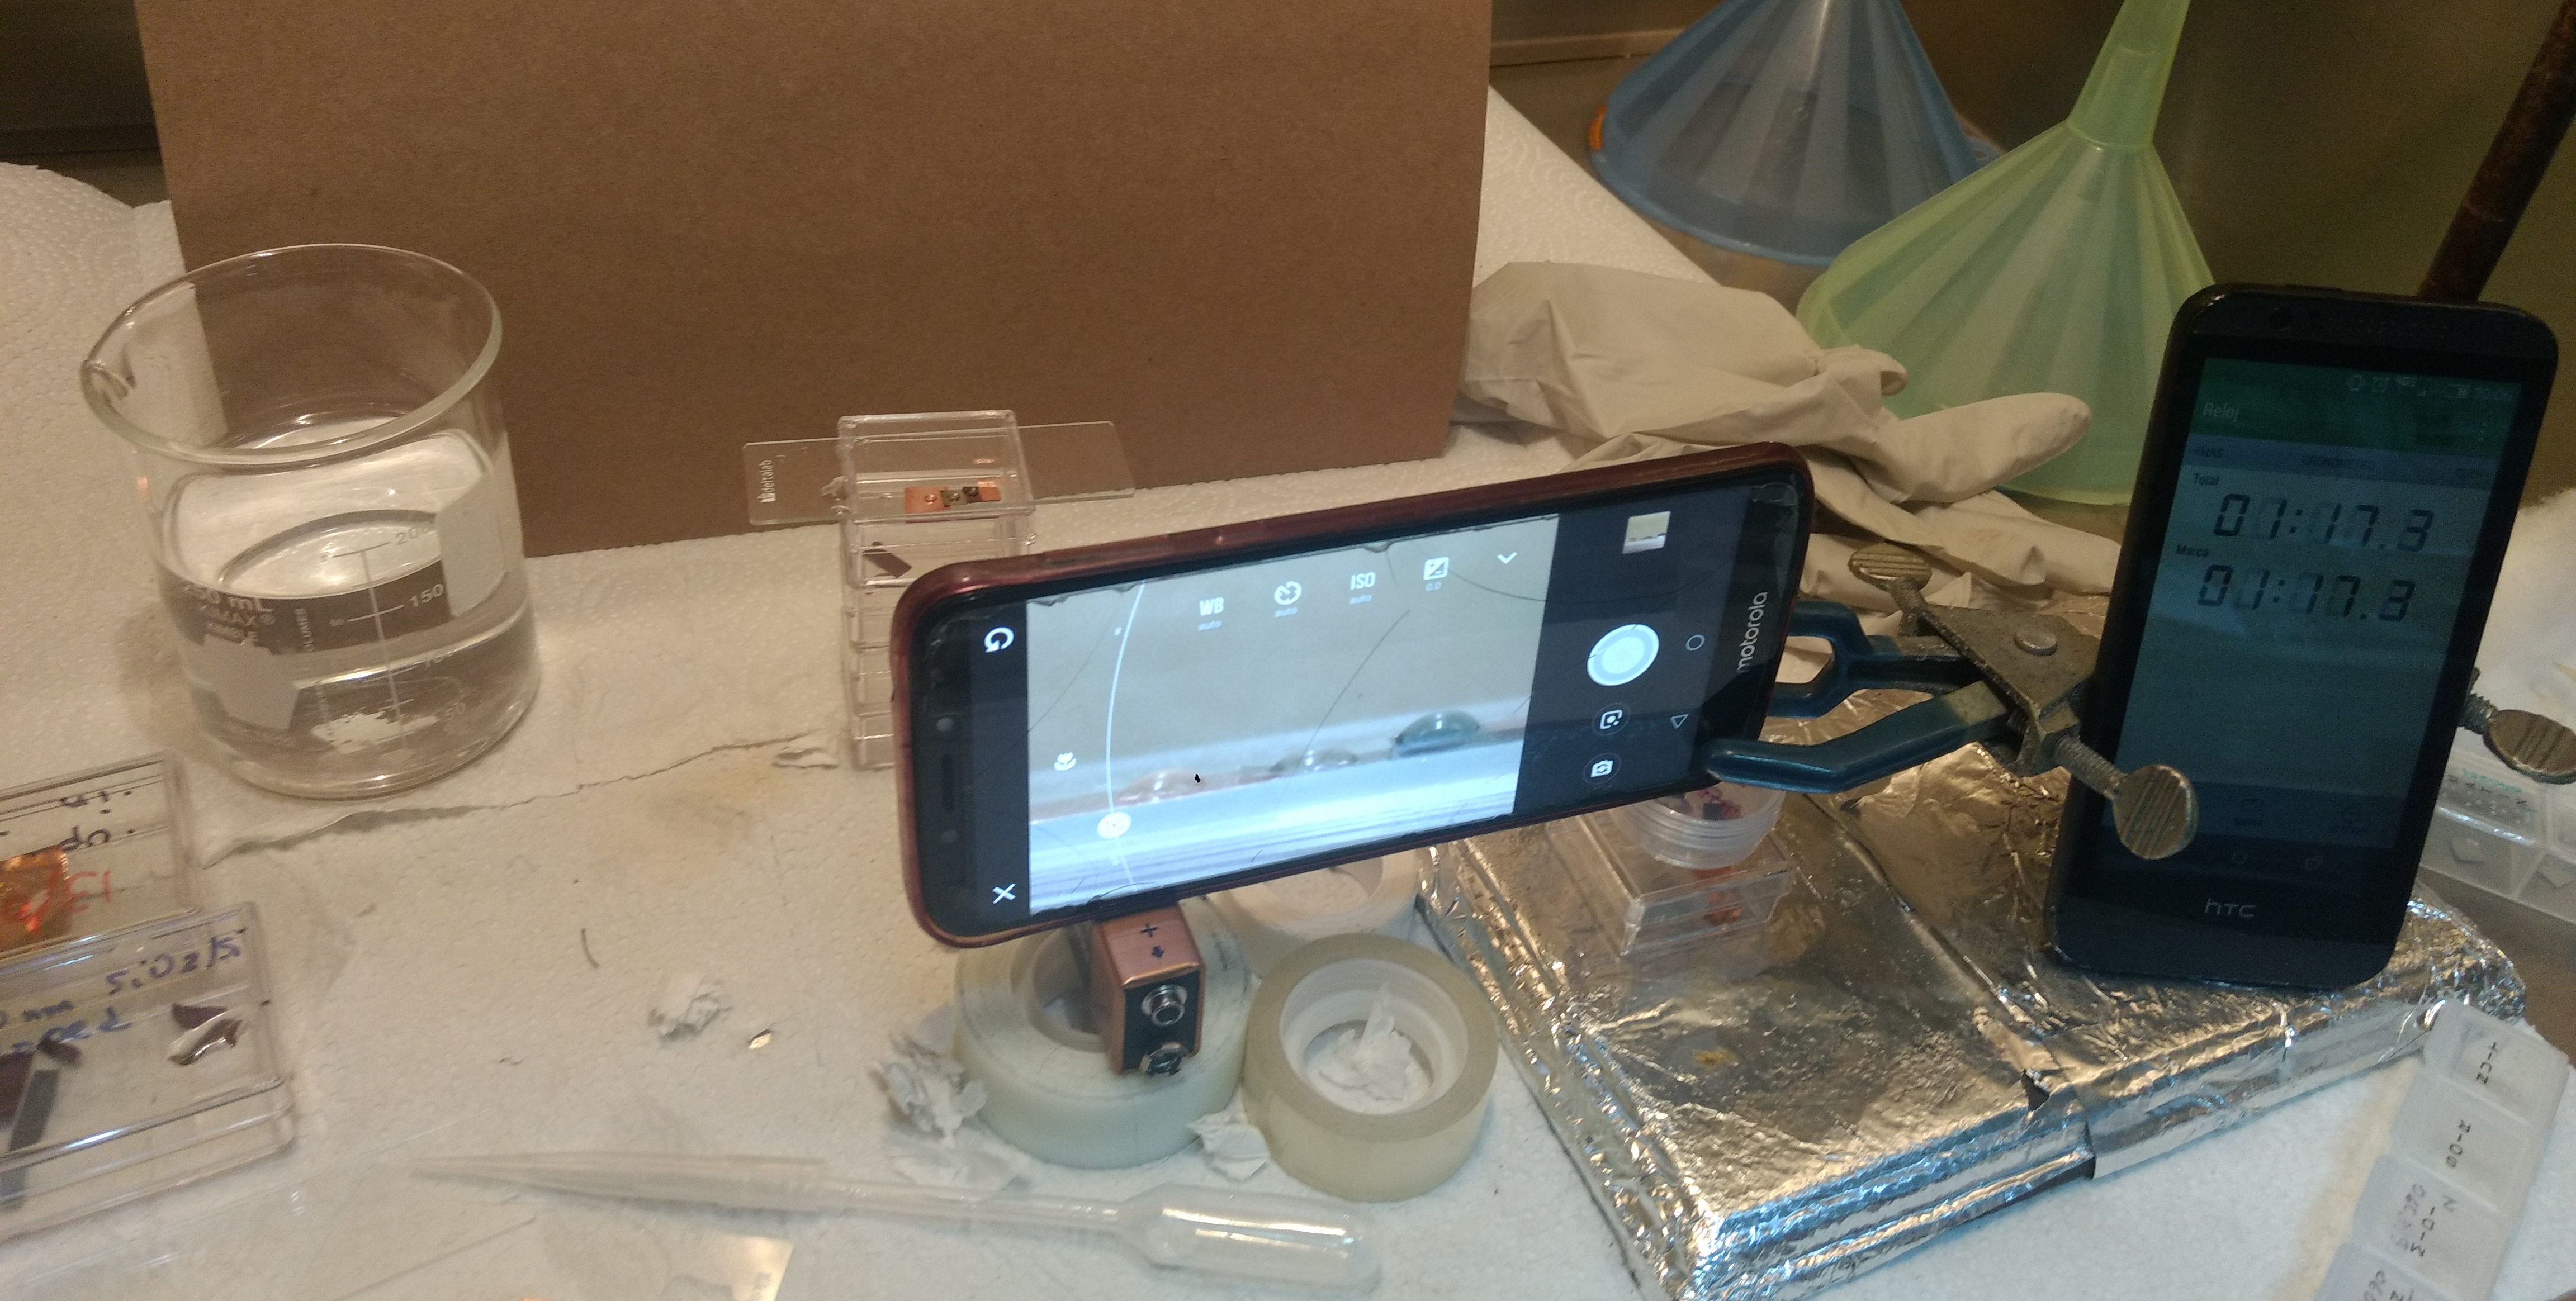
\includegraphics[scale=0.04]{SistemaGotas.jpg}
\caption{Se muestra el sistema utilizado para tomar las fotografías a las gotas cada 30 segundos .}
\end{figure}

Se colocaron gotas de agua desionizada sobre cada lámina de dos en dos, con y sin grafeno sobre ellas. La depositación de las gotas se hizo con una pipeta convencional, es decir, no se podía medir la cantidad de agua que se estaba depositando, por lo que se intetaba que las gotas quedaran del mismo tamaño. Imágenes de tomas de cada par de gotas analizadas se muestran en la Figura 12. Se tomaba foto a las gotas cada 30 segundos intentando que la toma fuera perpendicular al plano de las gotas.

\begin{figure}[hbtp]
\centering
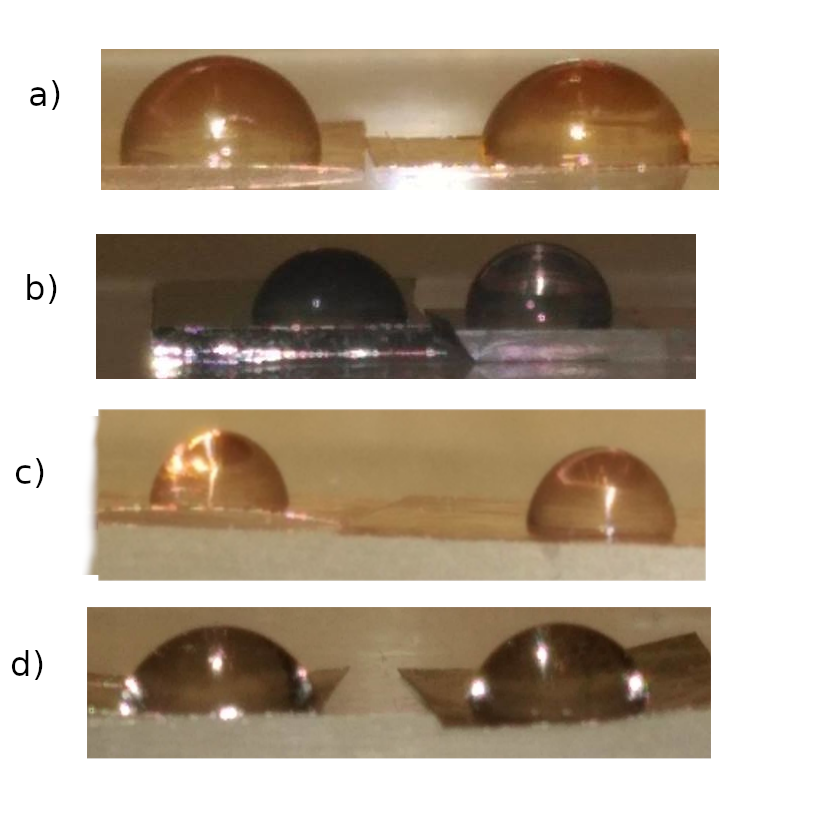
\includegraphics[scale=0.6]{Gotas_Todo.png}
\caption{a) Gotas de agua desionizada sobre cobre. b) Gotas de agua desionizada sobre silicio. c) Gotas de agua desionizada sobre cobre. d) Gotas de agua desionizada sobre paladio. A la derecha están las láminas con grafeno, a la izquierda las que no tienen grafeno.}
\end{figure}

Las imágenes obtenidas fueron analizadas para así obtener el ángulo de contacto de cada gota con cada material. Como se tomaron fotos cada 30 segundos, los cambios eran casi imperceptibles, por lo que se optó medir al menos cada 2 minutos el ángulo para que se pudiera analizar con menor error de medición.
%%%%%%%%%%%%%%%%%%%%%%%%%%%%%%%%%%%%%%%%%%%%%%%%%%%%%%%%%%%%%%%%%%%%%%%%%%%%%%
\section{Resultados y discusión}
Los resultados obtenidos del ángulo de corte del agua desionizada con cada lámina con y sin grafeno se muestran en la Figura 13. Se hicieron dos gráficas para el cobre como sustrato debido a las irregularidades que presentaba.

El ángulo de corte para cada material se muestra en la Tabla 1; se tomó en cuenta el ángulo de la primer fotografía tomada a cada material ya que al paso del tiempo no era confiable la medida debido a distintos factores ambientales.

\begin{figure}[h]
\centering
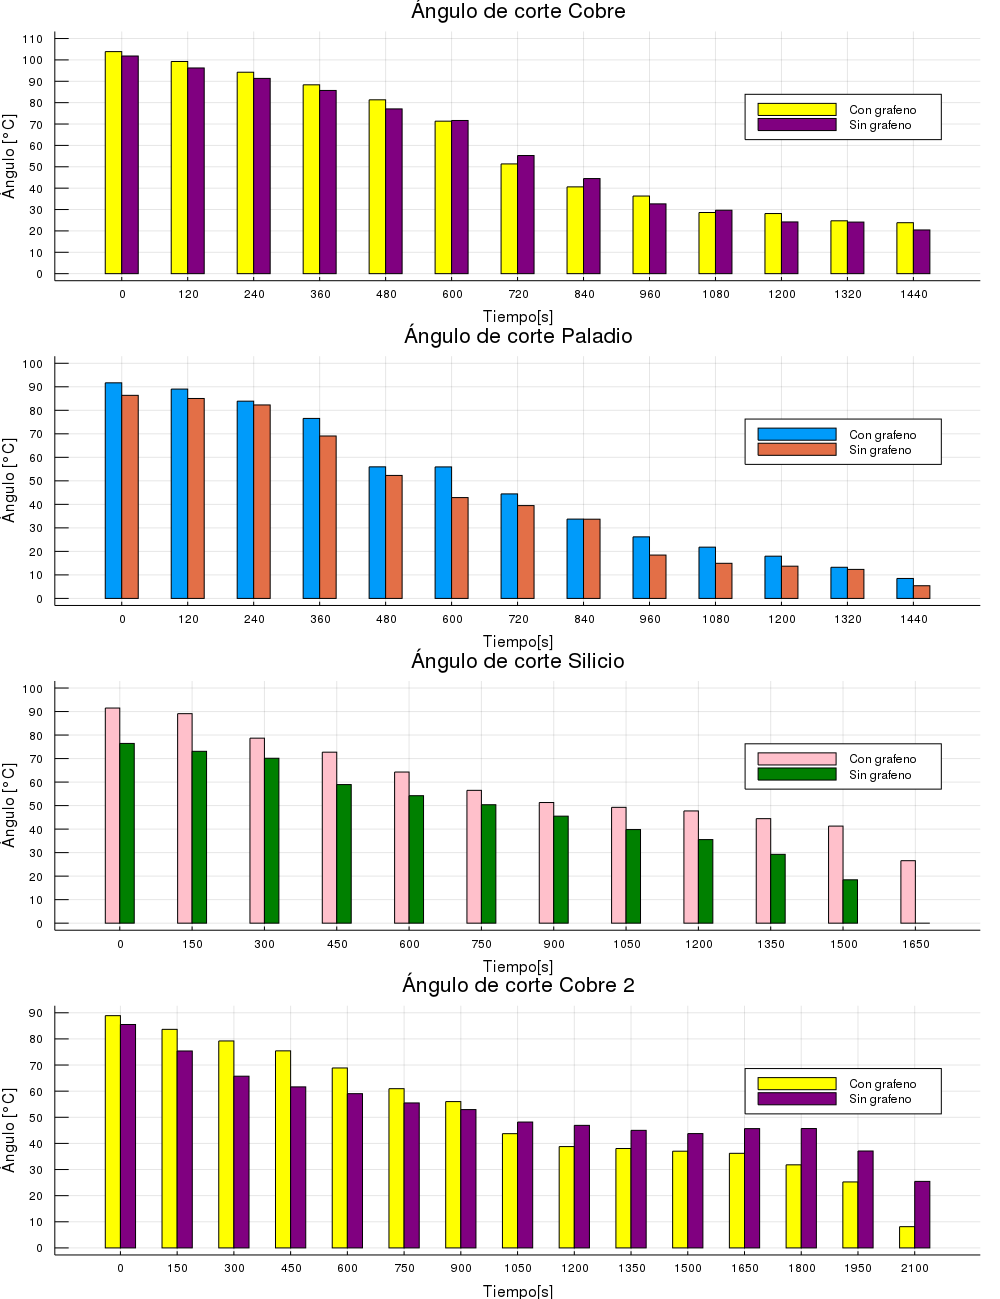
\includegraphics[scale=0.2]{Angulo_Corte_Todas.png}
\caption{Se muestran las gráficas de barras para cada tipo de sustrato, en cada gráfica individual se muestra cuando el sustrato tiene o no tiene grafeno.}
\end{figure}

En general, se nota que los ángulos de corte de la gota de agua desionizada son más grandes cuando hay grafeno sobre los sustratos, y además se observa que la gota que está sobre un sustrato con grafeno cae más despacio en general.

\begin{table}[h]
\begin{tabular}{|c|c|c|}
\hline 
 & \multicolumn{2}{c|}{Ángulo de Corte $\pm 0.0005^{o}$} \\ 
\hline 
 & Con grafeno & Sin grafeno \\ 
\hline 
\hline
Cobre & 101.821$^{o}$ & 103.878$^{o}$ \\ 
\hline 
Cobre 2 & 85.515$^{o}$ & 88.898$^{o}$ \\ 
\hline 
Paladio & 91.685$^{o}$ & 86.367$^{o}$ \\ 
\hline 
Silicio & 91.488$^{o}$ & 76.443$^{o}$ \\ 
\hline 
\end{tabular} 
\caption{Se muestran los ángulos de contacto de cada sustrato con y sin grafeno para la primera fotografía tomada para cada par de gotas.}
\end{table}

Con los ángulos mostrados en la Figura 13 se obtuvo el trabajo de adhesión debido a cada gota y sobre cada sustrato con y sin grafeno utilizando la ecuación \eqref{Young}. Los resultados obtenidos se muestran en la Figura 14.

\begin{figure}[h]
\centering
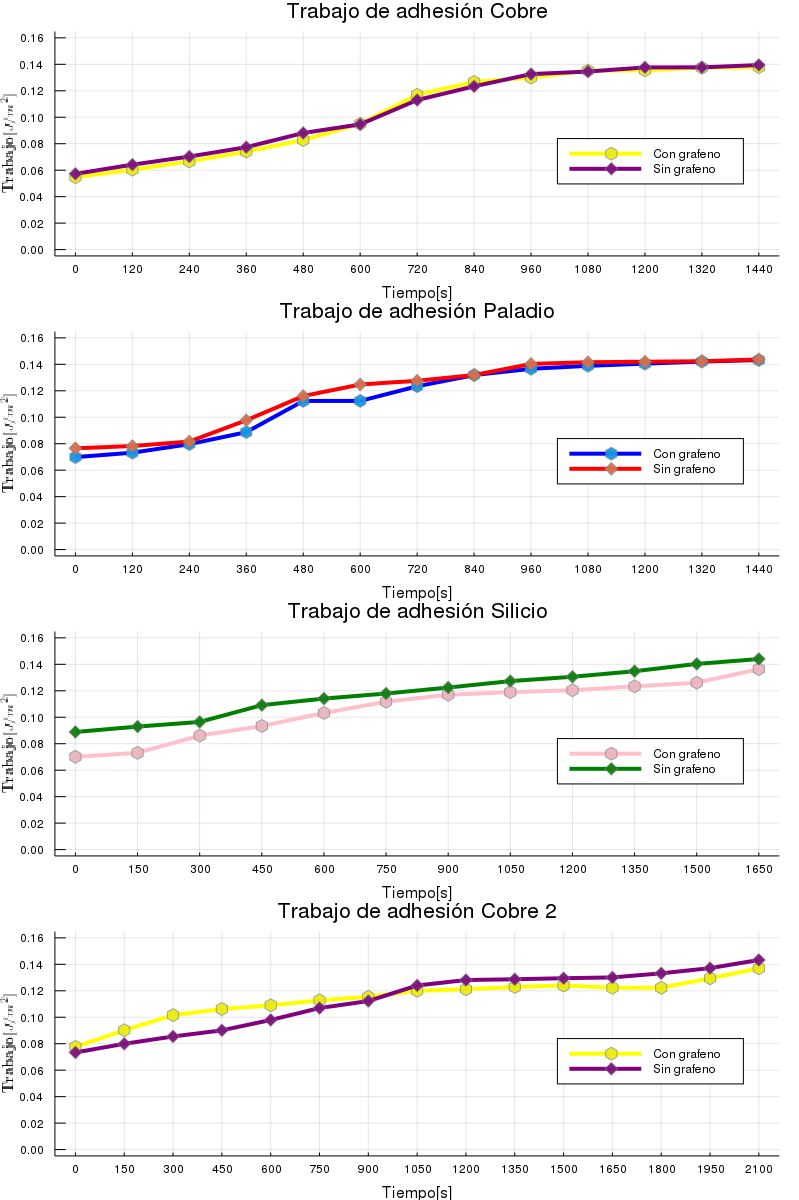
\includegraphics[scale=0.25]{graficas_Trabajo.png}
\caption{Trabajo de cohesión del agua para cada sustrato con y sin grafeno.}
\end{figure}

Se observa que en las gráficas para el cobre de la Figura 14 el trabajo medido varía, es decir, a veces se mide más cuando hay grafeno sobre el sustrato y a veces menos. En las gráficas de silicio y de paladio se nota que para cuando hay grafeno el trabajo es menor, por lo que la adhesión es menor, por lo que se observan propiedades hidrofóbicas.


%%%%%%%%%%%%%%%%%%%%%%%%%%%%%%%%%%%%%%%%%%%%%%%%%%%%%%%%%%%%%%%%%%%%%%%%%%%%%%
\section{Conclusiones}
En general, los sustratos con grafeno se observan más hidrofóbicos (incluso más que los reportados en la literatura), sin embargo, por las diferencias presentadas para el cobre se recomienda hacer más mediciones para poder hacer mejor estadística. Además, el tamaño usado para la gota no era constante ya que se usó una pipeta imprecisa que no marcaba mediciones tan pequeñas. Se recomienda usar una de 3 micro litros o menos, de modo que se tenga mas certeza de la medida y para que la gota no se desplome por su propio peso, causa que también intervino mucho en las pruebas junto con el poco control sobre las condiciones en donde se midió, como la presión, temperatura, luz, etc. También hay muchos errores al medir el ángulo, ya que se hizo con un programa computacional que depende completamente de la vista de quien esté analizando la muestra y de si el ángulo medido está realmente perpendicular a la cámara. Se recomienda que ya teniendo control sobre la medida de la gota, se hagan las pruebas gota por gota y no de dos en dos, además de una buena cámara con un angular grande y con enfoque manual, ésto para más claridad en las fotos y que sea más fácil y arbitrario medir en el programa computacional. Por último, se recomienda no hacer uso de flash al tomar las fotos y tener una buena iluminación que exponga bien las gotas pero evitando reflejos en los bordes donde se medirán los ángulos. Un fondo opaco es recomendable. 


%%%%%%%%%%%%%%%%%%%%%%%%%%%%%%%%%%%%%%%%%%%%%%%%%%%%%%%%%%%%%%%%%%%%%%%%%%%%%%
\begin{thebibliography}{99}
\bibitem{grafeno} Geim A. K., \textit{Graphene: Status and prospects}, Manchester Centre for Mesoscience and Nanotechnology, University of Manchester,  Oxford Road M13 9PL, Manchester, UK.

\bibitem{grafeno2} Ferrari A.C. et al., \textit{Raman Spectrum of Graphene and Graphene layers}, PHYSICAL REVIEW LETTERS, PRL 97, 187401, 2006: DOI: 10.1103/PhysRevLett.97.187401.

\bibitem{WCA1} Taherian F. et al., \textit{What is the Contact Angle of Water on Graphene}, ACS Publications, DOI: 10.1021/la304645w, Langmuir 2013, 1457 - 1465.

\bibitem{WCA2} Shin Y. J. et al., \textit{Surface-energy engineering of graphene}. Langmuir 2010, 26, 3798 - 3802.

\bibitem{WCA3} Rafiee J. et al., \textit{Wetting transparency of graphene}, Nat. Mater, 2012, 11, 217 - 222.

\bibitem{WCA4} Shih C. J. et al., \textit{Breakdown in the wetting transparency of graphene}, Phys. Rev. Lett. 2012, 109, 176101.

\bibitem{WCA5} Wang S. R. et al. \textit{Wettability and surface free energy of graphene films}, Langmuir 2009, 25, 11078 - 11081.

\bibitem{WCA6} Orlova E. et al., \textit{Investigation of drop dynamic contact angle on copper surface}, EPJ Web of Conferences82, 01053, DOI: 10.1051/epjconf/20158201053,  EDP Sciences, 2015.

\bibitem{WCA7} Tadros M. E. et al., \textit{Adsorption and Contact Angle Studies I. Water on Smooth Carbon, Linear Polyethylene, and Stearic Acid-Coated Copper}, Journal of Colloid and Interface Science, Vol. 49, No. 2, November 1974.

\bibitem{WCA8} Zhuang Y.X. et al., \textit{Growth and properties of self-assembled monolayers on metals}, DOI: 10.1088/1742 - 6596/152/1/012029, Journal of Physics: Conference Series, 152, 12 - 29, 2009.

\bibitem{YoungD} Seveno D. et al., \textit{Young's Equation at the Nanoscale}, Physical Review Letters, DOI: 10.1103/PhysRevLett.111.096101, 0031-9007/13/111(9)/096101(4), American Physical Society, 2013.

\bibitem{CVD} Creighton J. R., \textit{Introduction to Chemical Vapor Deposition (CVD)}, ASM International, Albuquerque, 2001.

\bibitem{Raman1} Wall M., \textit{The Raman Spectroscopy of Graphene and the Determination of Layer Thickness}, , Thermo-Fisher Scientific, Application Note: 52252:1-5, 2011.

\bibitem{Raman2} Schrader B., \textit{Infrared and Raman Spectroscopy}, B. ed., VCH Publishers Inc.: New York, 1995; Chapter 4.

\bibitem{PaladioCVD} Gutierrez-Valdés A. et al., \textit{Graphene CVD on Pd Substrates}, F. Ciencias - IFUNAM, México 2019.

\end{thebibliography}
\end{document}